% UC Merced  PhD Dissertation Template
% (UCSD Mathematics Dissertation Template is modified according to the UC Merced guidelines by Lasith Adhikari. Not responsible for any issues regarding modifications. You are welcome to add/update if there is any missing requirernment)
%
% Please read the comments in this file and make appropriate edits.
% NOTE: Always refer to the ``Preperation and Submission Manual for 
% Doctoral Dissertations and Masters Theses for 20**'', where 20** is 
% the year of your graduation, for officiation preparations guidelines.
%
% If you desire more control, please see the attached files:
%   * ucsd.cls -- Class file
%   * uct10.clo, uct11.clo, uct12.clo -- Configuration files for font sizes 10pt,11pt,12pt
%
% CHANGELOG:
%   * Original file adapted from brockman.tex by JRB and RMR
%     to work with ucsd.cls



\documentclass[12pt,chapterheads]{UCMerced}



\usepackage{pdfpages}
\usepackage{natbib}

 
% documentclass options: default is 11pt, oneside, final.
% fonts: 10pt, 11pt, 12pt -- are valid for UCSD dissertations (now UC Merced).
% sides: oneside, twoside -- note that two-sided theses are not accepted by OGS
% mode: draft, final -- draft mode switches to single spacing, removes hyperlinks,
%                       and places a black box at every overfull hbox (check these before submission).
% chapterheads -- include this if you want your chapters to read:
% Chapter 1
% Title of Chapter
%
% instead of
%
% 1 Title of Chapter


% Include all packages you need here.  Some standard options are suggested below.

% GEOMETRY - This will force the use of Letter paper.
% Many TeX installations default to A4 paper.  The formatting
% of the thesis class file requires Letter, else the margins
% will be wrong when you go to print it (and OGS will complain).
% If your TeX implementation is not setup for Letter paper, and
% you cannot change it, uncommenting the following line may fix 
% problem.
% \usepackage[paper=letterpaper]{geometry}


%% AMS PACKAGES - Chances are you will want some or all of these if writing a math dissertation.
% \usepackage{amsmath, amscd, amssymb, amsthm}

%% GRAPHICX - This is the standard package for including graphics for latex/pdflatex.
% \usepackage{graphicx}

%% LATIN MODERN FONTS (replacements for Computer Modern)
% \usepackage{lmodern}
% \usepackage[T1]{fontenc}

%% INDEX
% Uncomment the following two lines to create an index: 
% \usepackage{makeidx}
% \makeindex
% You will need to uncomment the \printindex line near the
% bibliography to display the index.  Use the command
% \index{keyword} within the text to create an entry in the index
% for keyword.

%% HYPERLINKS
% To create a PDF with hyperlinks, you need to include the hyperref package.
% THIS HAS TO BE THE LAST PACKAGE INCLUDED!
% Note that the options plainpages=false and pdfpagelabels exist
% to fix indexing associated with having both (ii) and (2) as pages.
% Also, all links must be black according to OGS.
% See: http://www.tex.ac.uk/cgi-bin/texfaq2html?label=hyperdupdest
% Note: This may not work correctly with all DVI viewers (i.e. Yap breaks).
% \usepackage[colorlinks=true, pdfstartview=FitV, linkcolor=black, citecolor=black, urlcolor=black,plainpages=false,pdfpagelabels]{hyperref}
% \hypersetup{ pdfauthor = {Your Name Here}, pdftitle = {The Title of The Dissertation}, pdfkeywords = {Keywords for Searching}, pdfcreator = {pdfLaTeX with hyperref package}, pdfproducer = {pdfLaTeX}}

\def\gal{{\tt galacticus}~}
\def\tides{{\tt T1DES}~}
\def\nsphere{{\tt NSphere}~}
\def\galns{{\tt galacticus}}
\def\pyh{{\tt PyHalo}~}
\def\pyhns{{\tt PyHalo}}
\def\cat{Caterpillar }
\def\catns{Caterpillar}
\def\symphony{Symphony }
\def\symphonyns{Symphony}
\def\col{{\tt colossus}~}
\def\colns{{\tt colossus}}
\def\astropy{{\tt astropy}~}
\def\astropyns{{\tt astropy}}
\def\subgen{{\tt subgen}~}
\def\subgenns{{\tt subgen}}
\def\sigsub{{$\Sigma_{\mathrm{sub}}$}}
\def\fssigsub{{$f_{\mathrm{s}} \cdot \Sigma_{\mathrm{sub}}$}}
\def\hanetal{\citet{10.1093/mnras/stv2900}~}
\def\hanetalns{\citet{10.1093/mnras/stv2900}}

\newcommand{\note}[1]{\textcolor{red}{\uppercase{#1}}}

\newcommand{\reffig}[1]{Figure \ref{#1}}

\newcommand{\refsec}[1]{Section \ref{#1}}
\newcommand{\refchap}[1]{Chapter \ref{#1}}
\newcommand{\refappendix}[1]{Appendix \ref{#1}}
\newcommand{\reftable}[1]{Table \ref{#1}}
\newcommand{\refeq}[1]{Eq. \ref{#1}}



\begin{document}

%% REQUIRED FIELDS -- Replace with the values appropriate to you
\title{Dark Matter Substructure}
% No symbols, formulas, superscripts, or Greek letters are allowed
% in your title.

\author{Charles Gannon}
\degreeyear{2017}
\degree{Doctor of Philosophy} 
% Master's Degree theses will NOT be formatted properly with this
% file.

\field{Physics}

\numberofmembers{4} % |chair|  + |othermembers| (do not count co-chair) % change here

\chair{Dr. Sarah R. Loebman}
% Uncomment the next line iff you have a Co-Chair
%\cochair{Professor Cochair Semimaster} 

\memberone{Dr. Anna Nierenber}
\membertwo{Dr. Andrew  Benson}
\memberthree{Dr. Lin Tian}

% Uncomment the next line iff you have more member
%\memberthree{Professor First Name Last Name 3}
%\memberfour{Professor First Name Last Name 4}
%\memberfive{Professor First Name Last Name 5}
%\membersix{Professor First Name Last Name 6}



\begin{frontmatter}
\makefrontmatter % The title, copyright, and signature pages.

%% DEDICATION
% You have three choices here:
%   1. Use the ``dedication'' environment.   Put in the text you want,
%   and you'll get a perfectly respectable dedication page.
%
%   2. Use the ``mydedication'' environment.  If you don't like the
%   formatting of option 1, use this environment and format things
%   however you wish.
%
%   3. If you don't want a dedication, it's not required.


\begin{dedication} % The style file will format this for you.
  
\end{dedication}

% \begin{mydedication} % You are responsible for formatting here.
%   \vspace{1in}
%   \begin{flushleft}
% 	To me.
%   \end{flushleft}
%   
%   \vspace{2in}
%   \begin{center}
% 	And you.
%   \end{center}
% 
%   \vspace{2in}
%   \begin{flushright}
% 	Which equals us.
%   \end{flushright}
% \end{mydedication}


%% EPIGRAPH
%  The same choices that applied to the dedication apply here.

\begin{epigraph} % The style file will position the text for you.
  \emph{A careful quotation\\
  conveys brilliance.}\\
  ---Smarty Pants
\end{epigraph}

% \begin{myepigraph} % You position the text yourself.
%   \vfil
%   \begin{center}
%     {\bf Think! It ain't illegal yet.}
% 
% 	\emph{---George Clinton}
%   \end{center}
% \end{myepigraph}

\tableofcontents
\listoffigures  % Uncomment if you have any figures
\listoftables   % Uncomment if you have any tables


%% ACKNOWLEDGEMENTS
%  While technically optional, you probably have someone to thank.
%  Also, a paragraph acknowledging all coauthors and publishers (if
%  you have any) is required in the acknowledgements page and as the
%  last paragraph of text at the end of each respective chapter. See
%  the OGS Formatting Manual for more information.

\begin{acknowledgements} 
 Thanks to whoever deserves credit for Blacks Beach, Porters Pub, and
 every coffee shop in Merced. 

 Thanks also to hottubs.
\end{acknowledgements}


%% VITA
%  A brief vita is required in a doctoral thesis. See the OGS
%  Formatting Manual for more information.
\begin{vitapage}
\begin{vita}
  \item[2002] B.~S. in Mathematics \emph{cum laude}, University of Southern North Dakota, Hoople
  \item[2002-2007] Graduate Teaching Assistant, University of California, Merced
  \item[2007] Ph.~D. in Mathematics, University of California, Merced
\end{vita}
\begin{publications}
  \item Your Name, ``A Simple Proof Of The Riemann Hypothesis'', \emph{Annals of Math}, 314, 2007.
  \item Your Name, Euclid, ``There Are Lots Of Prime Numbers'', \emph{Journal of Primes}, 1, 300
	B.C.
\end{publications}
\end{vitapage}

%% Abstract
% There does not seem to be a maximum length. From the OGS Formatting
% Manual: ``The abstract may continue on to a second page.''

\begin{abstract}
 Dark matter is thought to comprise the majority of the mass budget of the universe, with dark matter estimated to account for nearly $85\%$ of the total mass of the universe \cite{collaboration2020planck}. 
 Despite it's abundance, the nature of dark matter remains elusive.
 While Large scale cosmological probes such as Planck \cite{collaboration2020planck} and surveys of the spatial and mass function distributions of galaxies \cite{white1978core,white1991galaxy,de2008high,weinberg2015cold} have provided decisive evidence for an empirical model of dark matter that is cold and collisionless on the largest scale (CDM), the behavior of dark matter on the sub-galactic scale remains an area of active investigation and vigorous debate; one may hope that hints towards the underlying nature of dark matter can be found in this regime.
 A promising way to probe the physics of dark matter on the sub-galactic dark matter halos is by using anomalous flux ratios of quadruply lensed quasars. 
 In these systems, a light from a quasar passes through a central galaxy and is gravitationally lensed, producing four observable images. 
 Due to the non-linear nature of the dependence of flux ratios on the second derivative of the potential, information about dark matter on the sub galactic can be extracted from the flux ratios \cite{10.1093/mnras/stz3480}; several studies have used these methods to place constraints on Warm Dark Matter \cite{10.1093/mnras/stz3480, nadler2021dark} as well as self-interaction of dark matter \cite{2023PhRvD.107j3008G} without the need for luminous tracers required by many other dark matter probes.  
 In this work, study simulations and models of dark matter to develop informed priors on dark matter models to support strong gravitational lensing studies.
 We split this in two sections: first we explore developing informed priors on the projected number density of subhalos within lensing halos, then we explore developing a new simulation pipeline for 
 
 Perturbations in the density of dark matter gravitationally collapse into objects known as dark matter halos \cite{press1974formation}; understanding how these perturbations grow and evolve is important for placing constrains on dark matter models.  
 In this work, we focus in particular on subhalos: halos evolving under the gravitational field of a host. 
 N-body simulations suggest that subhalos account for $5$--$20\%$ of the total number of halos near the lensed images in projection with the subhalo to isolated halo ratio depending strongly on redshift \citep{10.1093/mnras/stu2673, 10.1093/mnras/sty159}; although subhalos are subdominant in , \citet{gilman2024turbocharging} showed that uncertainty in tidal stripping of models is a major source of uncertainty in strong gravitational lensing studies. 
 Subhalos can be numerically challenging to study: subhalos can lose $>99\%$ of their mass due to tidal stripping, leaving the subhalo prone to artificial noise in N-body simulations and possibly artificially disrupting, which would fictitiously lower the number of subhalos predicted by these simulations {\color{red} CITE THE CDM REMMENANTS PAPER HERE}.
 To overcome these challenges we use the state-of-the-art semi-analytic \gal {\color{red} CITATION HERE} model tuned to ultra high resolution N-body simulations that minimize the effects of artificial disruption.
 Using this model we develop informed priors on the projected halo mass function expected by lensing studies, develop models for the scaling of the halo mass function with redshift and halo mass and explore the tidal effects of a realistically evolving potential of a central galaxy. 
 We find that a factor of $\sim 2$ accounts for theoretical uncertainties in the subhalos mass function and find that for current lesning studies the central galaxy has a currently negligible impact on the projected number density of substructure. 

 Recent inferences on the sub-galactic from direct gravitational imaging the potential of lenses \cite{vegetti2010detection, minor2021unexpected, tajalli2025sharp} have provided evidence for anomalously dense dark matter halos compared to CDM predictions.
 Although these results have been hotly debated and solutions within the CDM framework have been proposed \cite{he2025not}, the intriguing possibility remains that these results hint at physics beyond CDM; possible explanations include a class of alternate dark matter models with non-negligible self-interaction on the sub-galactic scales, called self-interacting dark matter (SIDM).
 In these models, dark matter self-interaction facilitates the conduction of heat within the halo; due to the negative heat capacity of self-gravitating systems, runaway heat transfer can occur leading to the halo gravothermally collapsing, leading to extremely dense collapsed remnants at the end of their evolution \cite{tulin2018dark,adhikari2025astrophysical}.
 3-D N-body simulations, which are traditionally the primary method of studying dark matter halos are computationally expensive especially in the core collapse regime; tidal mass loss amplifies this challenge by requiring a larger number of particles to resolve the halo initially, often requiring tens of thousands of core hours to properly resolve core collapse  even in idealized simulations. 
 In this work, we develop a pipeline to simulate the evolution of idealized SIDM subhalos in 1-D with realistic tidal evolution; by simulating subhalos evolution in 1-D, we are able to simulate SIDM physics much more computationally efficiently than the 3D case, resulting in over an order of magnitude speed up in some case enabling previously infeasible exploration of SIDM model space. 
 Using our models we explore the core collapse rates for a wide range for a wide range of SIDM cross sections for a realistic population of halos. 
 

 
 %In \refchap{chap:alp}
 
 
 
 

    
\end{abstract}
\end{frontmatter}


%% DISSERTATION
\chapter{Introduction}
\chapter{Introduction}\label{chap:intro}
Chapter 1 test

\chapter{A Lensing Perspective}\label{chap:alp}
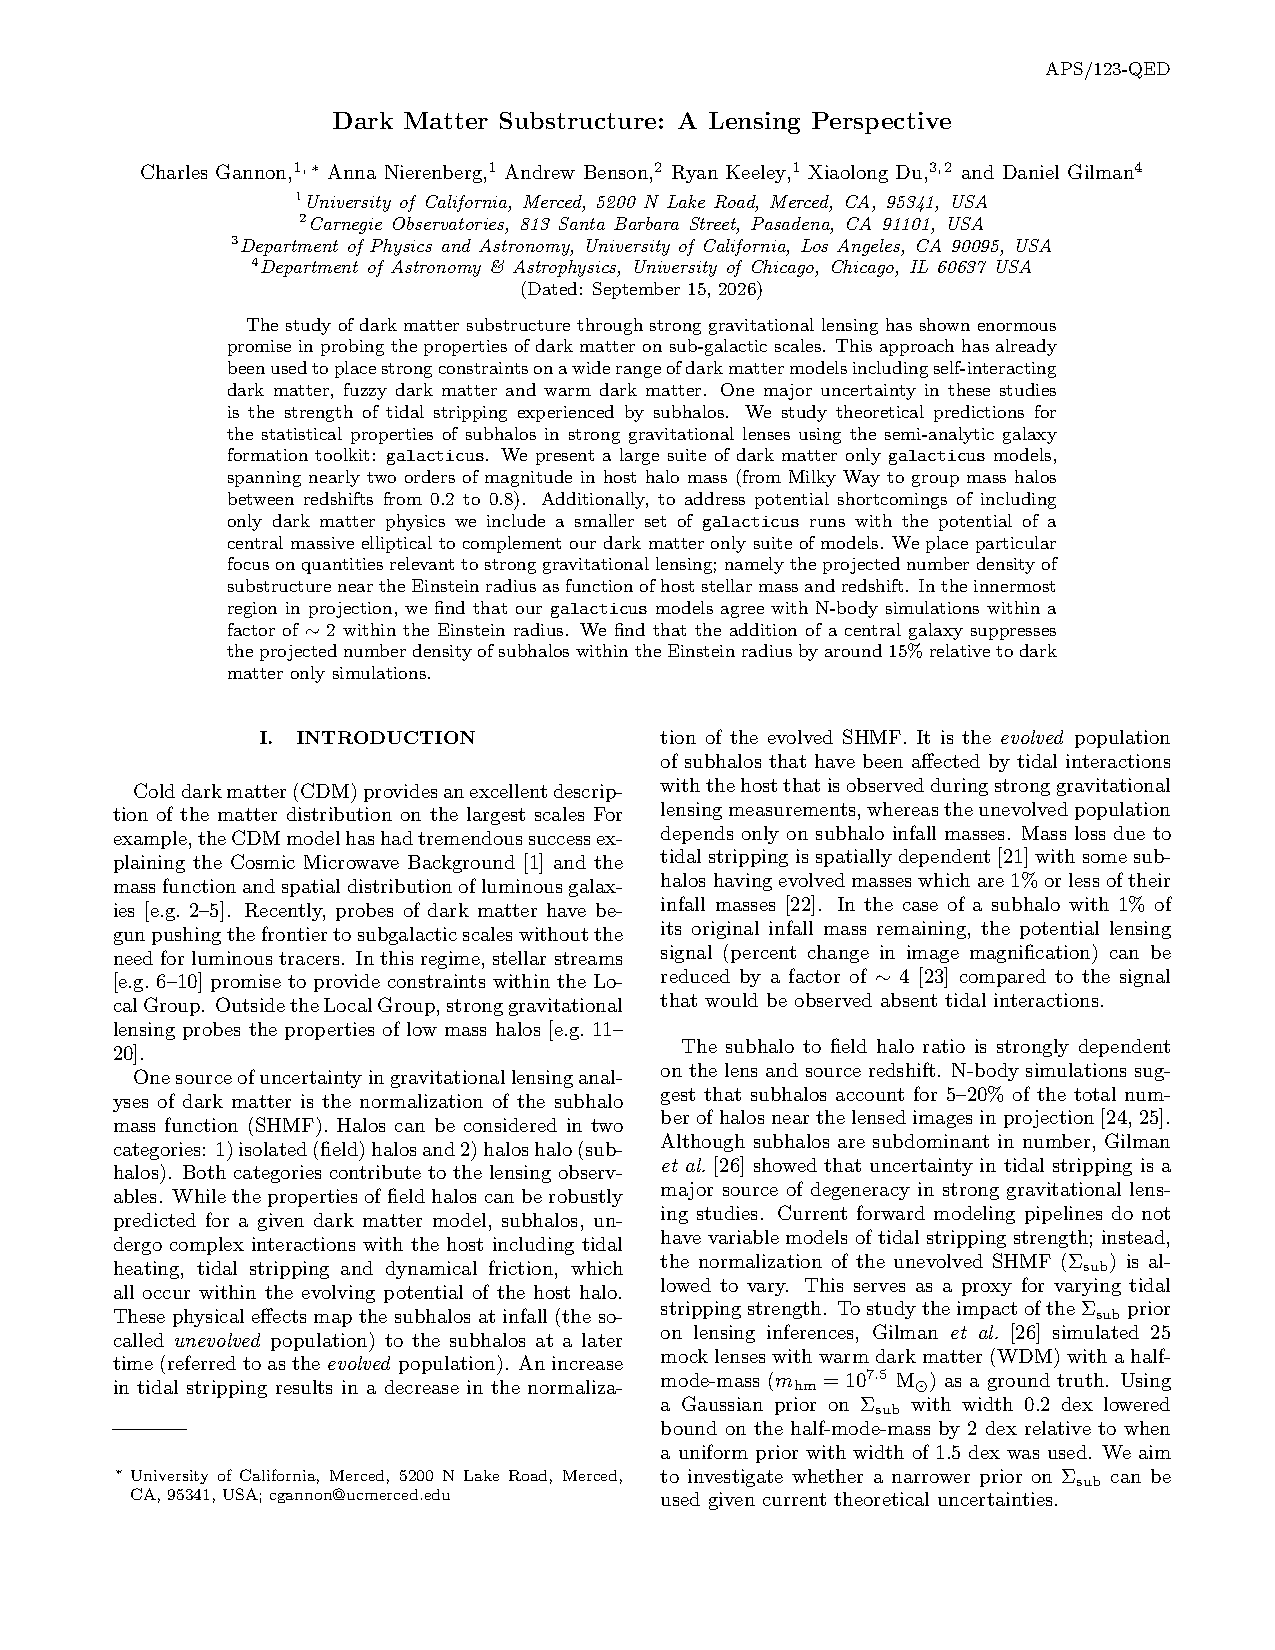
\includepdf[pages=-]{papers/A_Lensing_Perspective.pdf}

\chapter{T1DES in SIDM}
\chapter{T1DES in SIDM}\label{chap:tides}
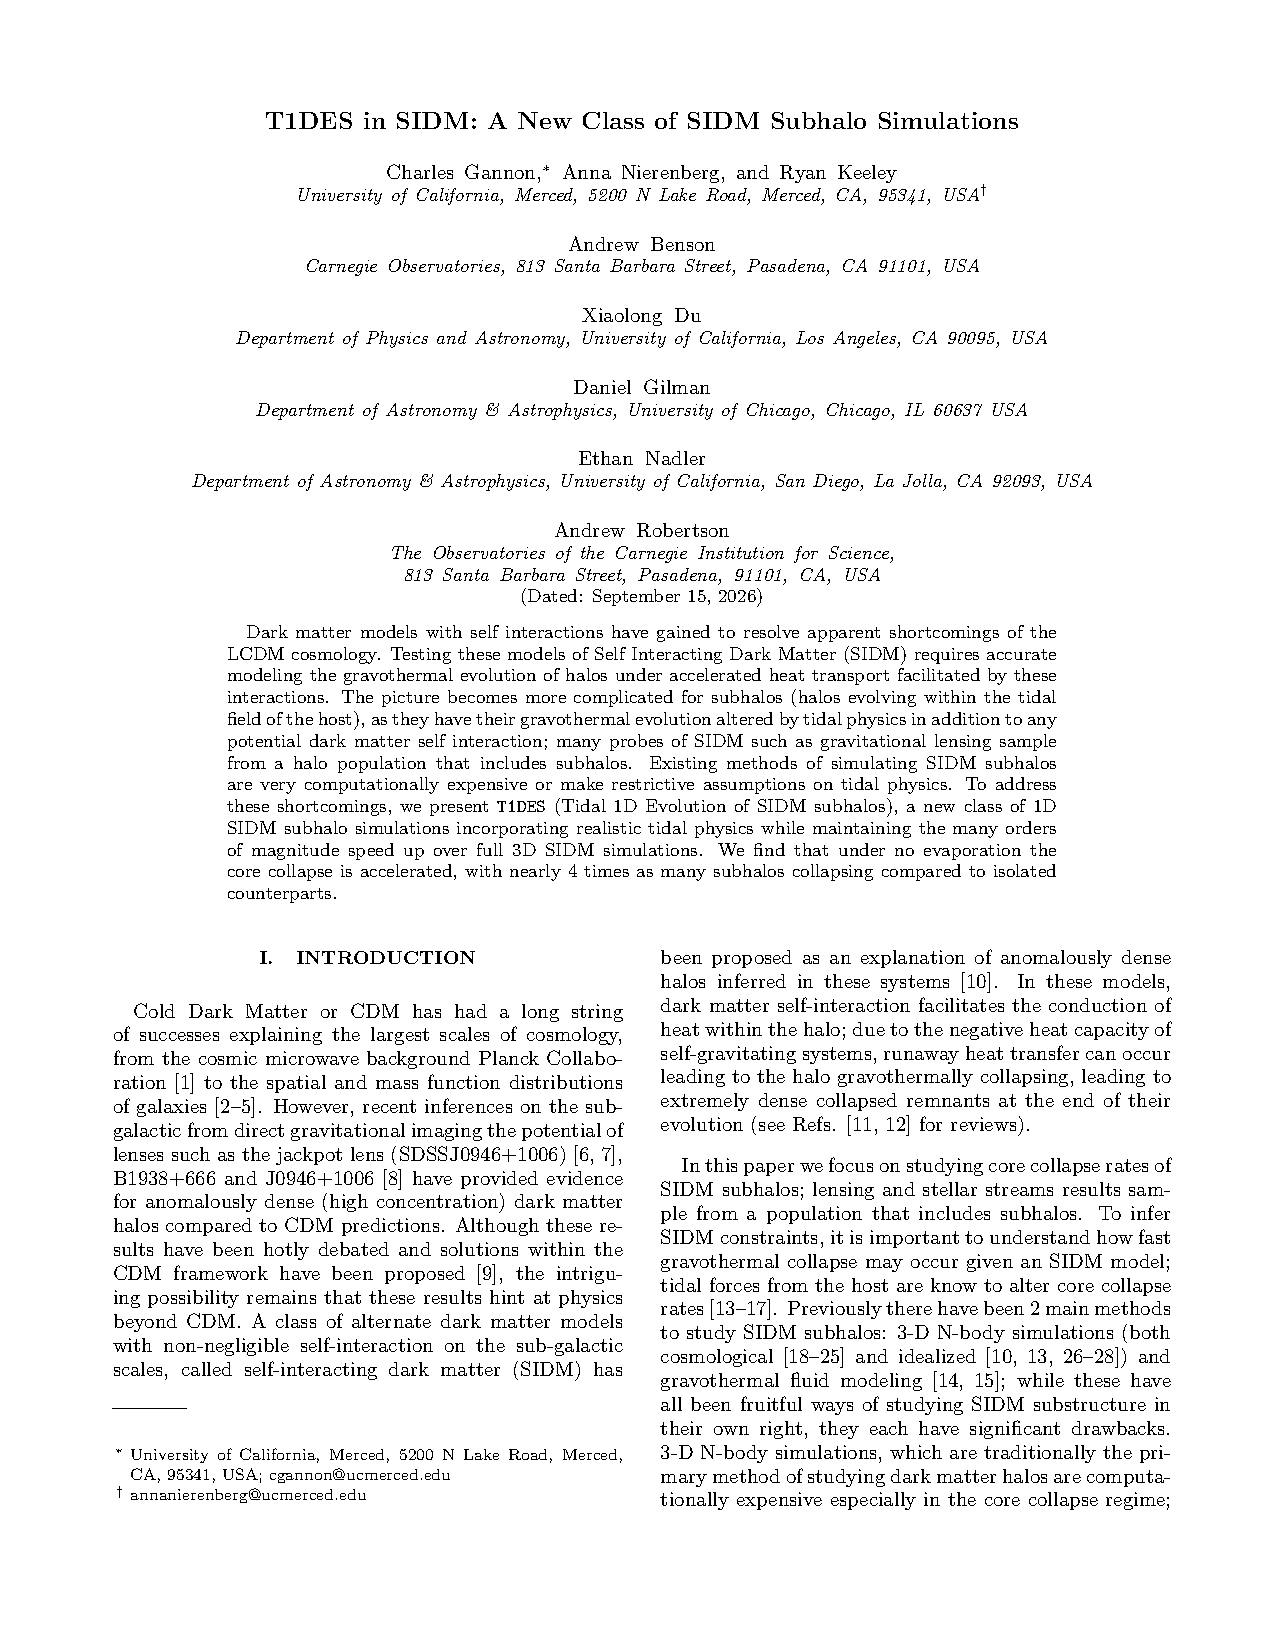
\includepdf[pages=-]{papers/tides.pdf}

\chapter{Conclusion}
\chapter{Conclusion}
In this work, we study the substructure of group mass lensing like halos.
We work toward developing informed priors on 



\appendix
%\chapter{Final notes}
  %Remove me in case of abdominal pain.

%% END MATTER
% \printindex %% Uncomment to display the index
% \nocite{}  %% Put any references that you want to include in the bib 
%               but haven't cited in the braces.
\bibliographystyle{plain}  %% This is just my personal favorite style. 
%                              There are many others.
\bibliography{mybib}  %% This looks for the bibliography in myrefs.bib 
%                          which should be formatted as a bibtex file.
\end{document}

